%!TEX root=../../main.tex

\section{Exercises}

% Chapter 6 exercises
% format adapted from inference_for_means
% problems drawn from OI 4 source files
%__________________
\subsection{Examining scatterplots}

% current commented numbers are from oi4, and from our sequence oibio

% oibio 1

% oi4 3

\eoce{\qt{Identify relationships, Part I\label{identify_relationships_1}} 
For each of the six plots, 
identify the strength of the relationship (e.g. weak, moderate, or 
strong) in the data and whether fitting a linear model would be 
reasonable.
\begin{center}
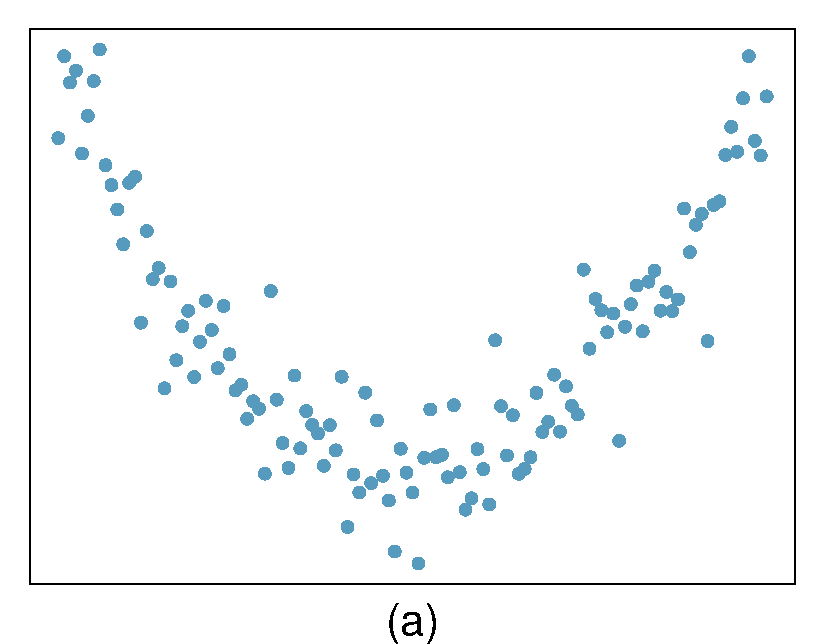
\includegraphics[width=0.32\textwidth]{ch_simple_linear_regression_oi_biostat/figures/eoce/identify_relationships_1/identify_relationships_u.pdf}
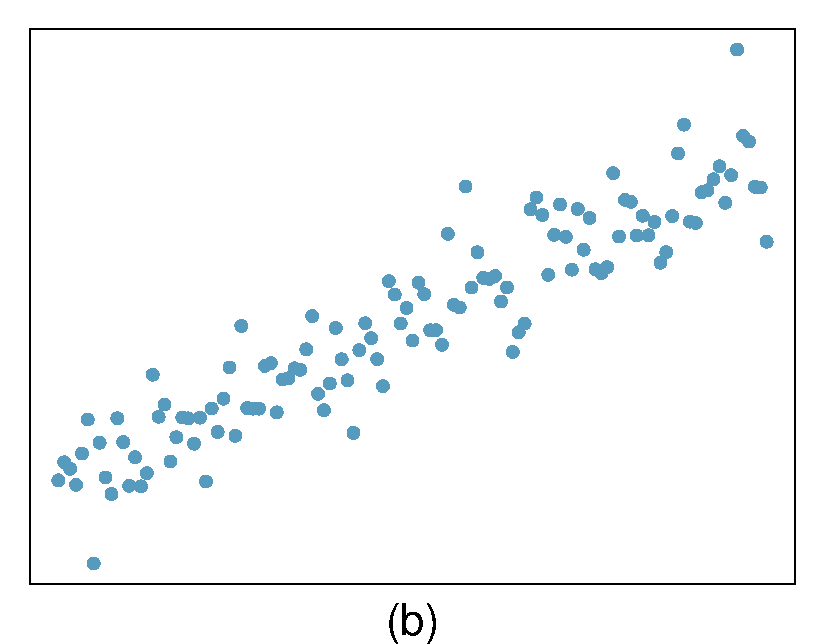
\includegraphics[width=0.32\textwidth]{ch_simple_linear_regression_oi_biostat/figures/eoce/identify_relationships_1/identify_relationships_lin_pos_strong.pdf}
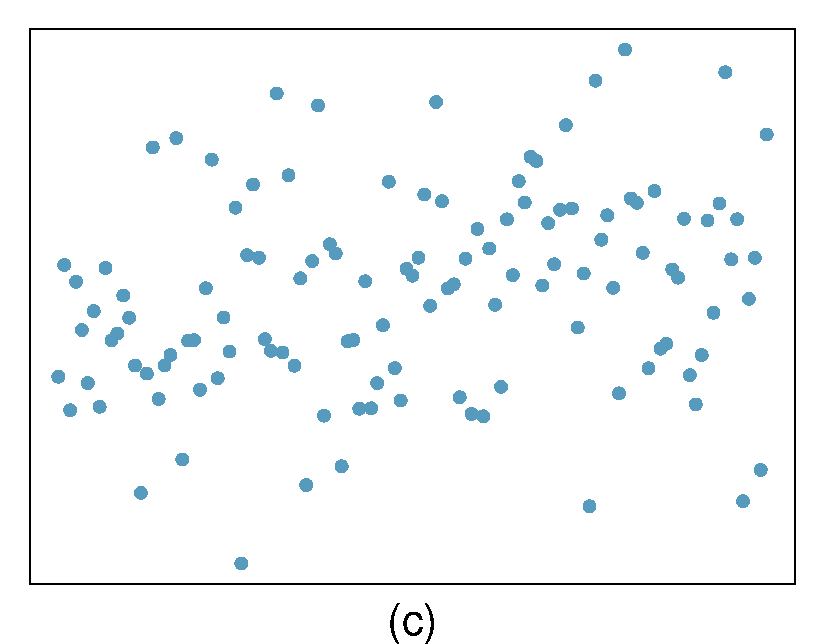
\includegraphics[width=0.32\textwidth]{ch_simple_linear_regression_oi_biostat/figures/eoce/identify_relationships_1/identify_relationships_lin_pos_weak.pdf}
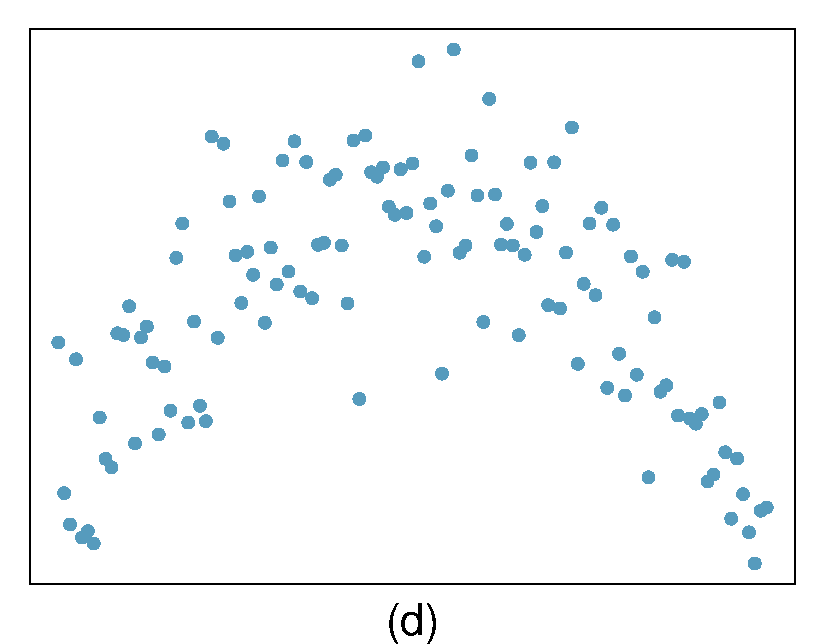
\includegraphics[width=0.32\textwidth]{ch_simple_linear_regression_oi_biostat/figures/eoce/identify_relationships_1/identify_relationships_n.pdf}
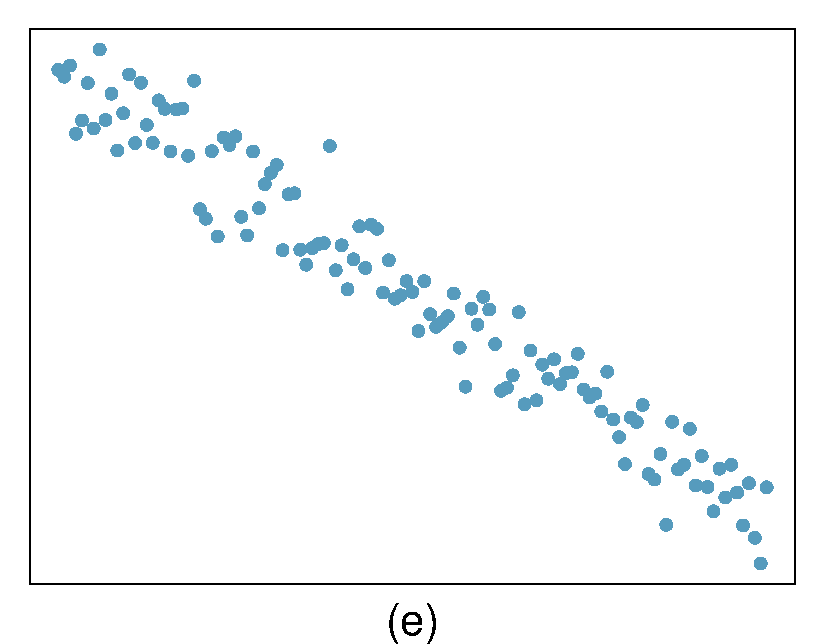
\includegraphics[width=0.32\textwidth]{ch_simple_linear_regression_oi_biostat/figures/eoce/identify_relationships_1/identify_relationships_lin_neg_strong.pdf}
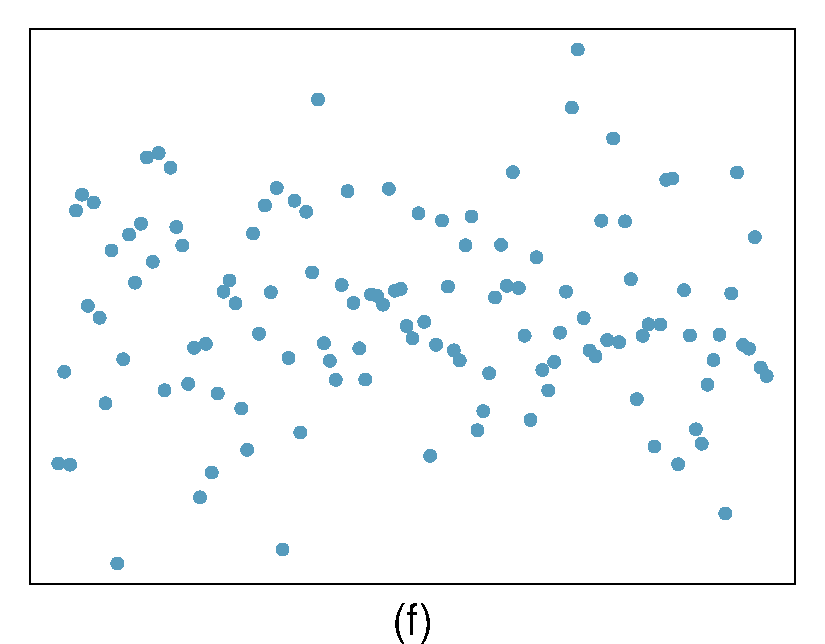
\includegraphics[width=0.32\textwidth]{ch_simple_linear_regression_oi_biostat/figures/eoce/identify_relationships_1/identify_relationships_none.pdf}
\end{center}
}{}

% \D{\newpage}

% oibio 2
% oi4 4

\eoce{\qt{Identify relationships, Part II\label{identify_relationships_2}} 
For each of the six plots, 
identify the strength of the relationship (e.g. weak, moderate, or 
strong) in the data and whether fitting a linear model would be 
reasonable.
\begin{center}
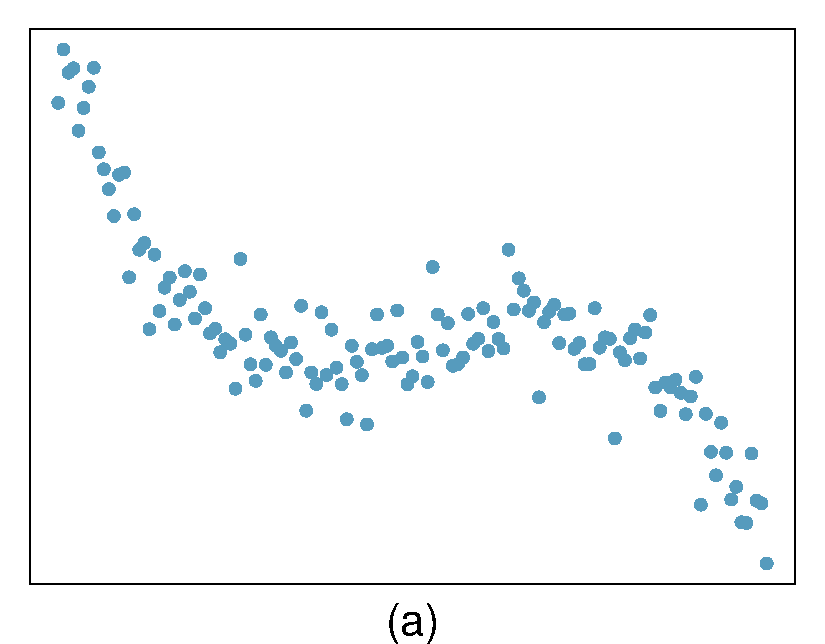
\includegraphics[width=0.32\textwidth]{ch_simple_linear_regression_oi_biostat/figures/eoce/identify_relationships_2/identify_relationships_s.pdf}
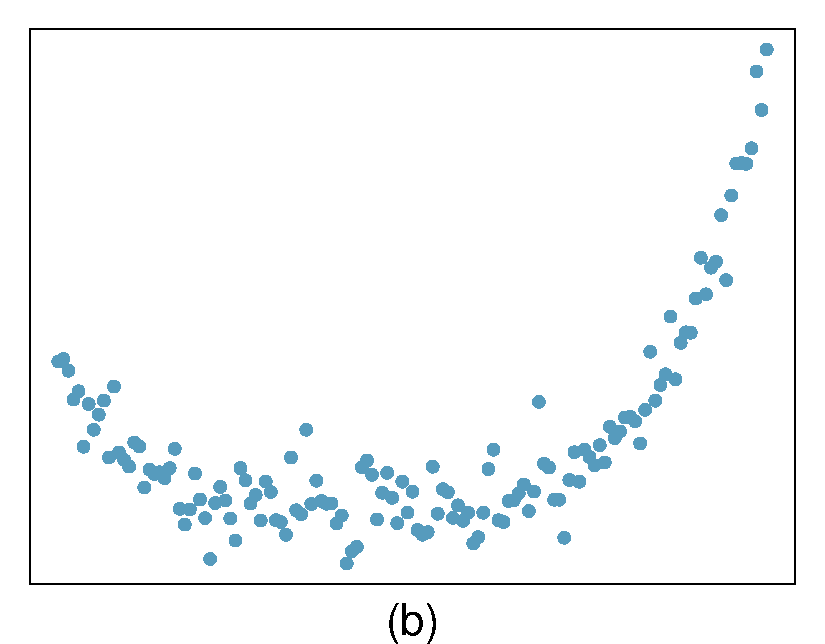
\includegraphics[width=0.32\textwidth]{ch_simple_linear_regression_oi_biostat/figures/eoce/identify_relationships_2/identify_relationships_hockey_stick.pdf}
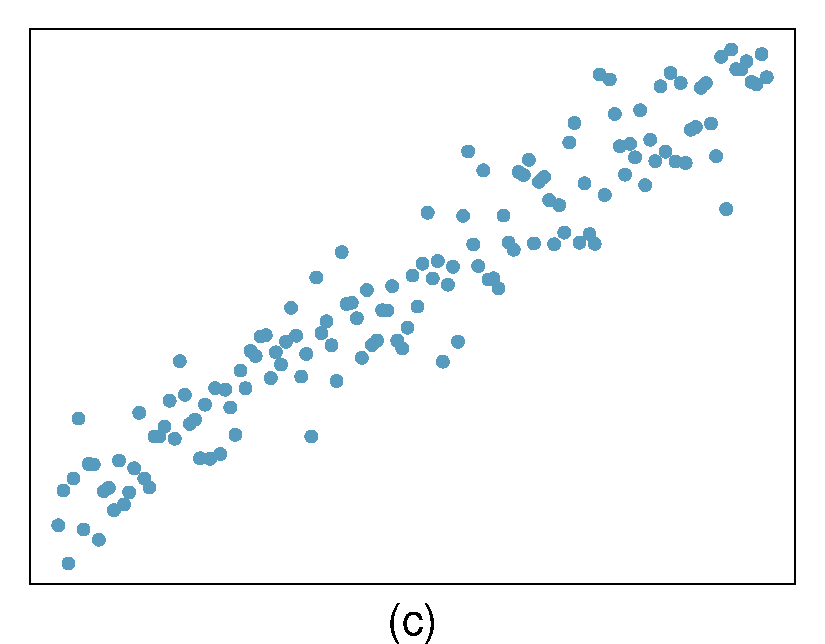
\includegraphics[width=0.32\textwidth]{ch_simple_linear_regression_oi_biostat/figures/eoce/identify_relationships_2/identify_relationships_pos_lin_strong.pdf}
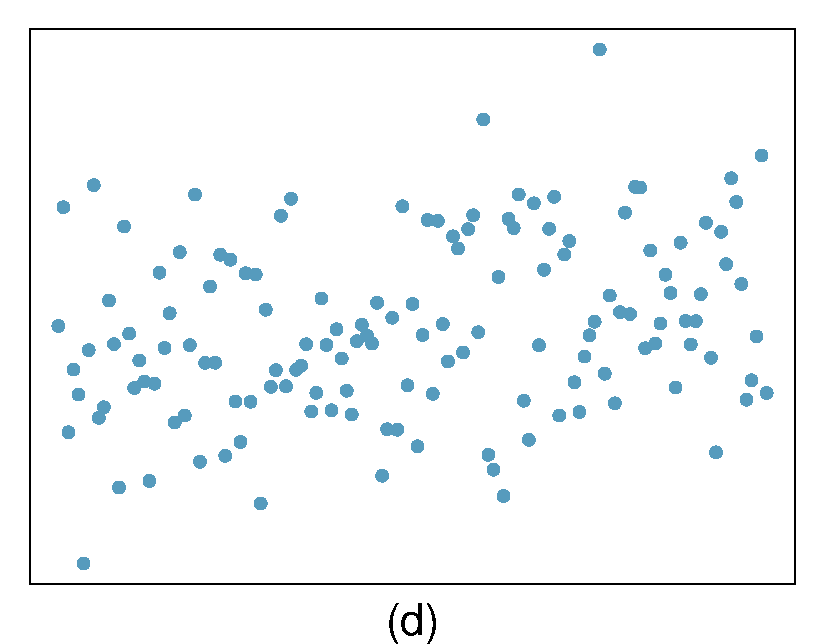
\includegraphics[width=0.32\textwidth]{ch_simple_linear_regression_oi_biostat/figures/eoce/identify_relationships_2/identify_relationships_pos_weak.pdf}
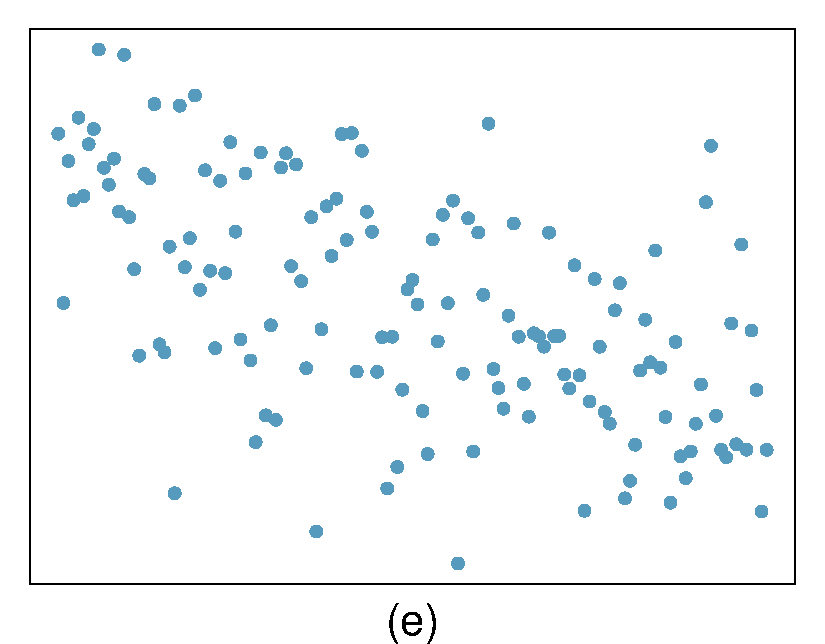
\includegraphics[width=0.32\textwidth]{ch_simple_linear_regression_oi_biostat/figures/eoce/identify_relationships_2/identify_relationships_pos_weaker.pdf}
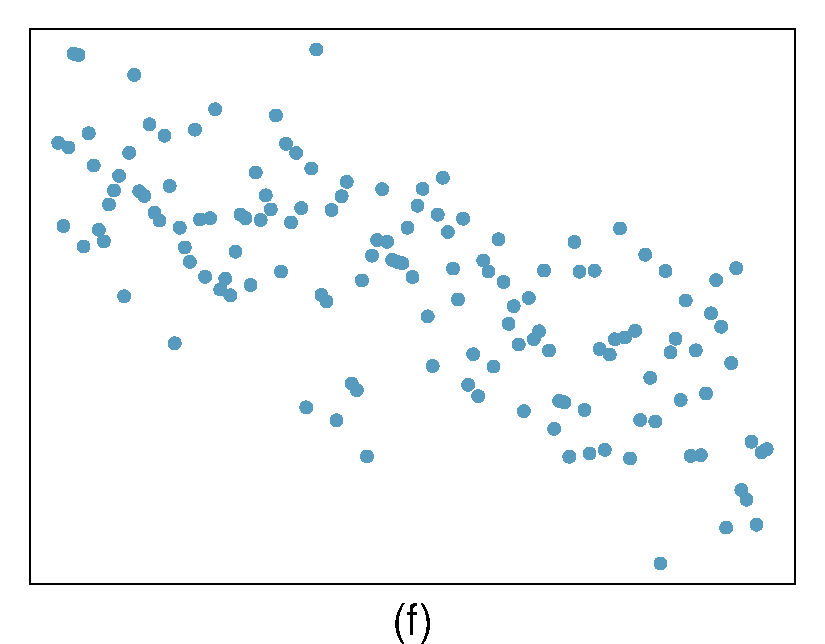
\includegraphics[width=0.32\textwidth]{ch_simple_linear_regression_oi_biostat/figures/eoce/identify_relationships_2/identify_relationships_neg_lin_weak.pdf}
\end{center}
}{}


\subsection{Estimating a regression line using least squares}

% oibio 3
% oi4 1

\eoce{\qt{Visualize the residuals\label{visualize_residuals}} 
The scatterplots shown below each have a 
superimposed regression line. If we were to construct a residual plot 
(residuals versus $x$) for each, describe what those plots would look 
like.
\begin{center}
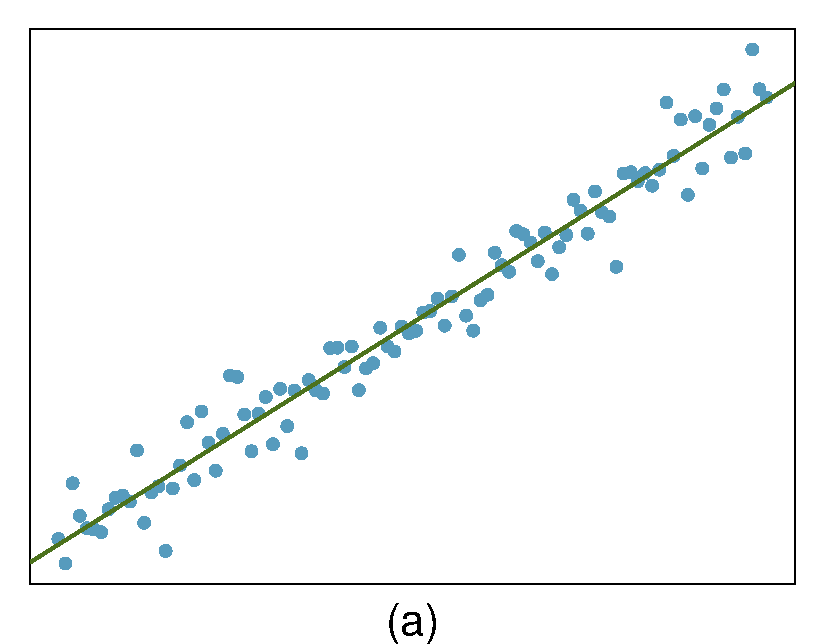
\includegraphics[width=0.42\textwidth]{ch_simple_linear_regression_oi_biostat/figures/eoce/visualize_residuals/visualize_residuals_linear.pdf} 
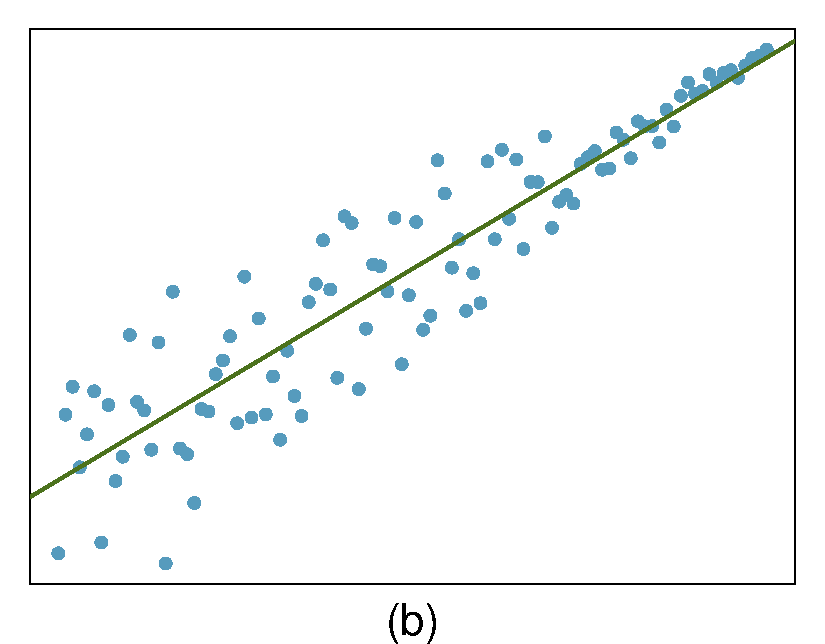
\includegraphics[width=0.42\textwidth]{ch_simple_linear_regression_oi_biostat/figures/eoce/visualize_residuals/visualize_residuals_fan_back.pdf}
\end{center}
}{}

% oibio 4

% oi4 13

\eoce{\qt{Body measurements, Part I\label{body_measurements_shoulder_height_corr_units}} 
Researchers studying anthropometry collected body girth measurements and 
skeletal diameter measurements, as well as age, weight, height and gender 
for 507 physically active individuals.\footfullcite{Heinz:2003} The 
scatterplot below shows the relationship between height and shoulder 
girth (over deltoid muscles), both measured in centimeters.\vspace{3mm}

\noindent%
\begin{minipage}[c]{0.4\textwidth}
{\raggedright\begin{parts}
\item Describe the relationship between shoulder girth and height.
\item How would the relationship change if shoulder girth was measured 
in inches while the units of height remained in centimeters?
\end{parts}\vspace{20mm}}
\end{minipage}
\begin{minipage}[c]{0.1\textwidth}                  
$\:$\\
\end{minipage}
\begin{minipage}[c]{0.485\textwidth}
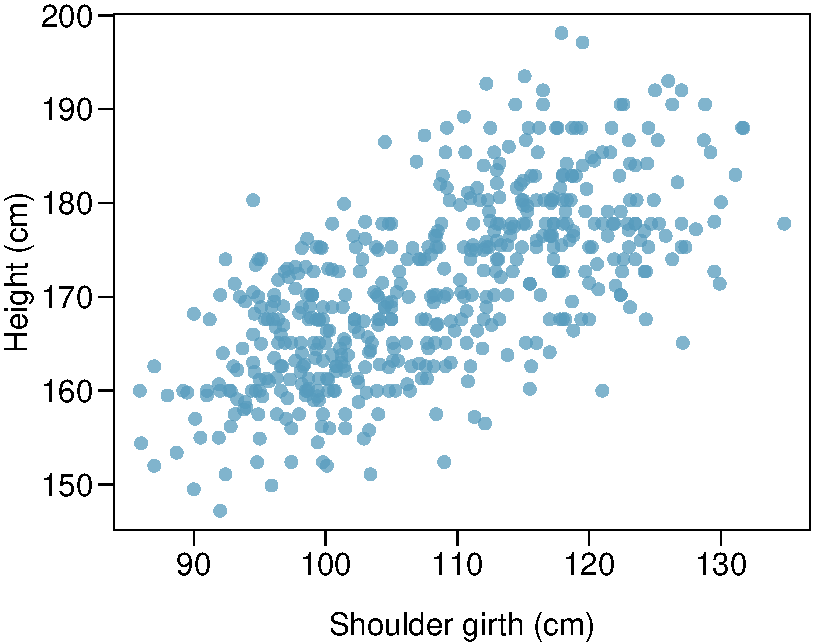
\includegraphics[width=\textwidth]{ch_simple_linear_regression_oi_biostat/figures/eoce/body_measurements_shoulder_height_corr_units/body_measurements_height_shoulder_girth.pdf}
\end{minipage}
}{}

% oibio 5

% oi4 14

\eoce{\qt{Body measurements, Part II\label{body_measurements_hip_weight_corr_units}} 
The scatterplot below shows the relationship between weight 
measured in kilograms and hip girth measured in centimeters 
from the data described in 
Exercise~\ref{body_measurements_shoulder_height_corr_units}.%
\vspace{3mm}

\noindent%
\begin{minipage}[c]{0.4\textwidth}
{\raggedright\begin{parts}
\item Describe the relationship between hip girth and weight.
\item How would the relationship change if weight was measured in pounds 
while the units for hip girth remained in centimeters?
\end{parts}\vspace{20mm}}
\end{minipage}
\begin{minipage}[c]{0.1\textwidth}
$\:$\\
\end{minipage}
\begin{minipage}[c]{0.485\textwidth}
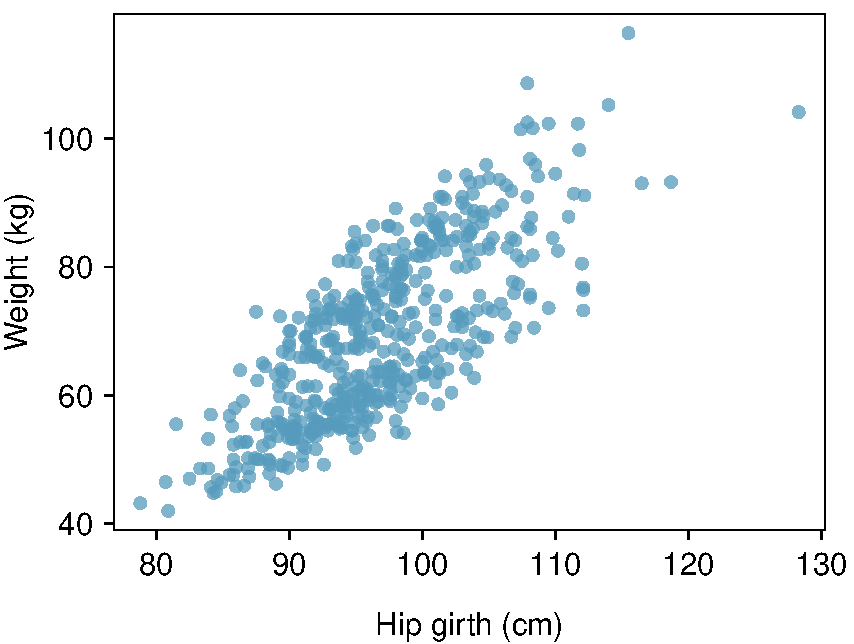
\includegraphics[width=\textwidth]{ch_simple_linear_regression_oi_biostat/figures/eoce/body_measurements_hip_weight_corr_units/body_measurements_weight_hip_girth.pdf}
\end{minipage}
}{}

% oibio 6

% oi4 19

\eoce{\qt{Over-under, Part I\label{residual_apple_weight}} Suppose we fit a 
regression line to predict the shelf life of an apple based on its weight. 
For a particular apple, we predict the shelf life to be 4.6 days. The 
apple's residual is -0.6 days. Did we over or under estimate the 
shelf-life of the apple? Explain your reasoning.
}{}

% oibio 7

%oi4  20

\eoce{\qt{Over-under, Part II\label{residual_sun_cancer}} Suppose we fit a 
regression line to predict the number of incidents of skin cancer per 
1,000 people from the number of sunny days in a year. For a particular 
year, we predict the incidence of skin cancer to be 1.5 per 1,000 people, 
and the residual for this year is 0.5. Did we over or under estimate 
the incidence of skin cancer? Explain your reasoning.
}{}

% oibio 8

% oi4 22

\eoce{\qt{Nutrition at Starbucks, Part I\label{starbucks_cals_carbos}} 
The scatterplot below shows the relationship between the number of 
calories and amount of carbohydrates (in grams) Starbucks food menu 
items contain.\footfullcite{data:starbucksCals} Since Starbucks only 
lists the number of calories on the display items, we are interested 
in predicting the amount of carbs a menu item has based on its 
calorie content.
\begin{center}
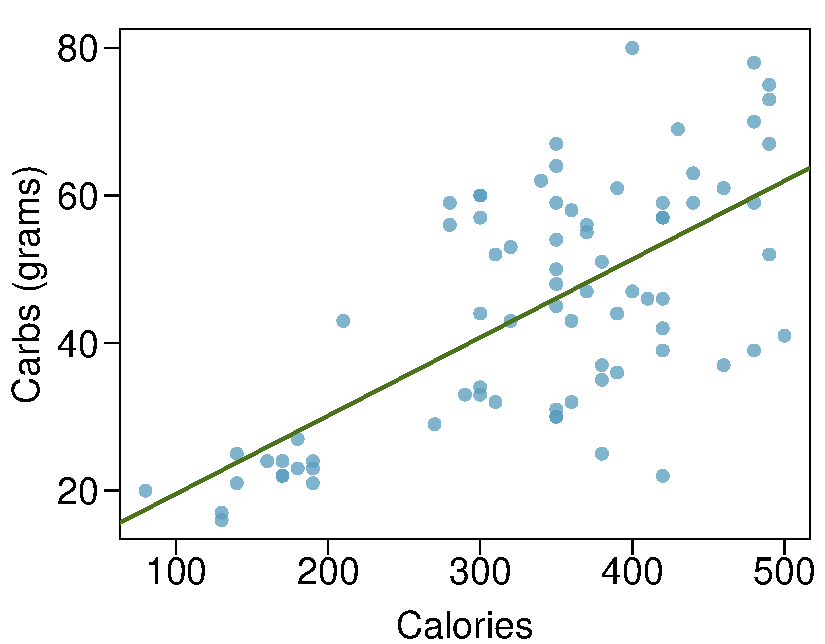
\includegraphics[width=0.32\textwidth]{ch_simple_linear_regression_oi_biostat/figures/eoce/starbucks_cals_carbos/starbucks_cals_carbos.pdf}
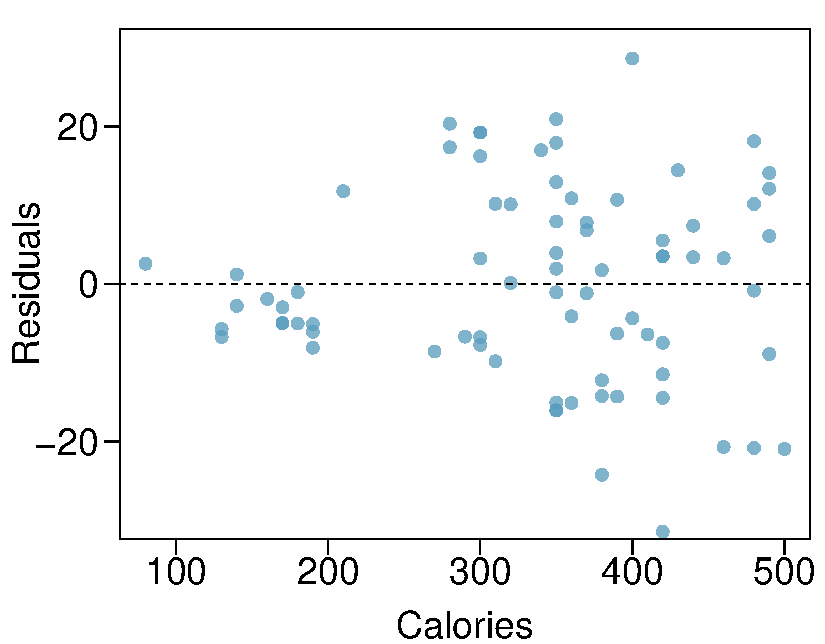
\includegraphics[width=0.32\textwidth]{ch_simple_linear_regression_oi_biostat/figures/eoce/starbucks_cals_carbos/starbucks_cals_carbos_residuals.pdf}
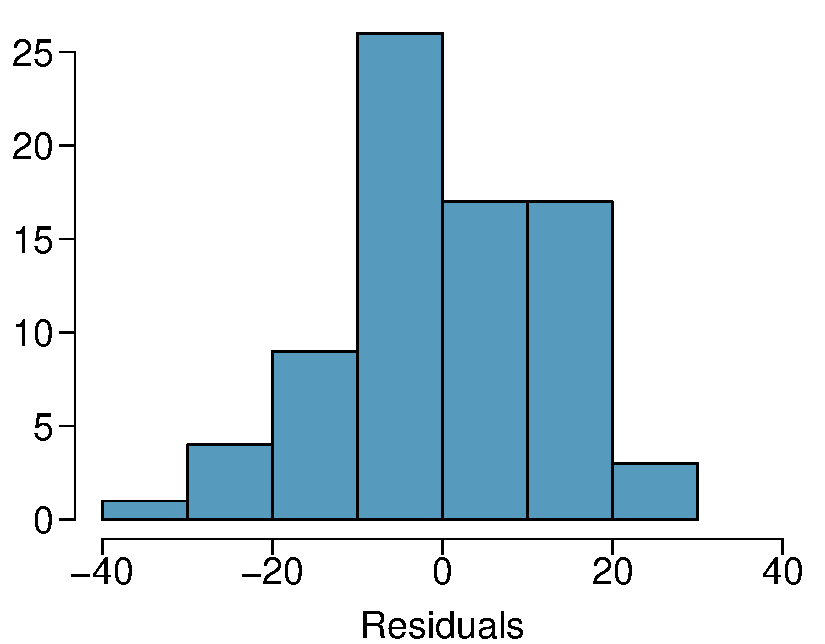
\includegraphics[width=0.32\textwidth]{ch_simple_linear_regression_oi_biostat/figures/eoce/starbucks_cals_carbos/starbucks_cals_carbos_residuals_hist.pdf}
\end{center}
\begin{parts}
\item Describe the relationship between number of calories and amount 
of carbohydrates (in grams) that Starbucks food menu items contain.
\item In this scenario, what are the explanatory and response 
variables?
\item Why might we want to fit a regression line to these data?
\item Do these data meet the conditions required for fitting a least 
squares line?
\end{parts}
}{}

\subsection{Interpreting a linear model}

% oibio 9
% oi4 24

\eoce{\qt{Body measurements, Part III\label{body_measurements_shoulder_height_reg}}
Exercise~\ref{body_measurements_shoulder_height_corr_units} introduces 
data on shoulder girth and height of a group of individuals. The 
mean shoulder girth is 107.20 cm with a standard deviation of 
10.37 cm. The mean height is 171.14 cm with a standard deviation 
of 9.41 cm. The correlation between height and shoulder girth is 0.67.
\begin{parts}
\item Write the equation of the regression line for predicting height.
\item Interpret the slope and the intercept in this context.
\item Calculate $R^2$ of the regression line for predicting height 
from shoulder girth, and interpret it in the context of the 
application.
\item A randomly selected student from your class has a shoulder 
girth of 100 cm. Predict the height of this student using the model.
\item The student from part~(d) is 160 cm tall. Calculate the 
residual, and explain what this residual means.
\item A one year old has a shoulder girth of 56 cm. Would it be 
appropriate to use this linear model to predict the height of this 
child?
\end{parts}
}{}


% oibio 10

% oi4 25

\eoce{\qt{Murders and poverty, Part I\label{murders_poverty_reg}} The following 
regression output is for predicting annual murders per million from 
percentage living in poverty in a random sample of 20 metropolitan 
areas.\\[2mm]
\begin{minipage}[c]{0.54\textwidth}
{\footnotesize
\begin{tabular}{rrrrr}
    \hline
            & Estimate  & Std. Error    & t value   & Pr($>$$|$t$|$) \\ 
    \hline
(Intercept) & -29.901   & 7.789         & -3.839    & 0.001 \\ 
poverty\%   & 2.559     & 0.390         & 6.562     & 0.000 \\ 
   \hline
\end{tabular} \\
$s = 5.512 \hfill R^2 = 70.52\% \hfill R^2_{adj} = 68.89\%$ 
}
\begin{parts}
\item Write out the linear model.
\item Interpret the intercept.
\item Interpret the slope.
\item Interpret $R^2$.
\item Calculate the correlation coefficient.
\end{parts}
\end{minipage}
\begin{minipage}[c]{0.02\textwidth}
$\:$\\
\end{minipage}
\begin{minipage}[c]{0.41\textwidth}
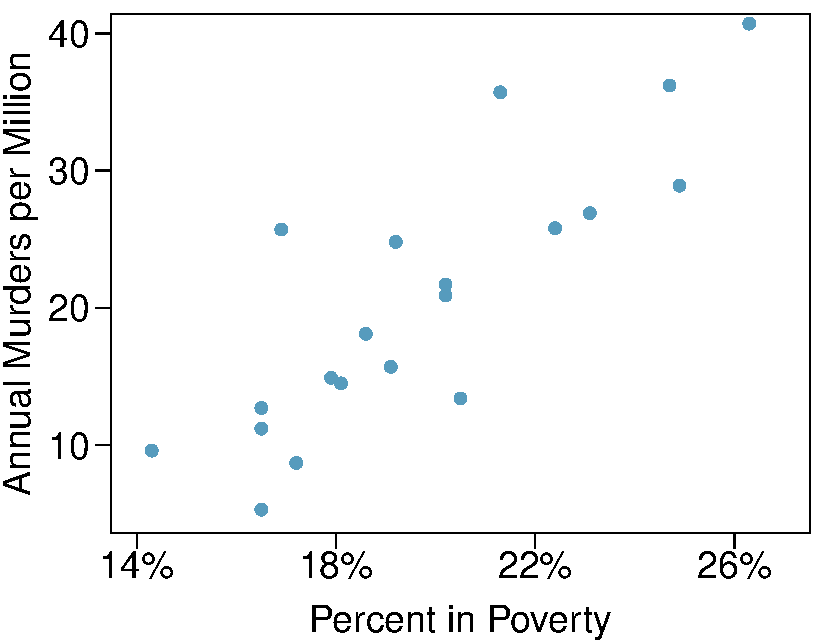
\includegraphics[width=\textwidth]{ch_simple_linear_regression_oi_biostat/figures/eoce/murders_poverty_reg/murders_poverty.pdf}
\end{minipage}
}{}

% oibio 11
% oi4 26

\eoce{\qt{Cats, Part I\label{cat_body_heart_reg}} The following regression output is 
for predicting the heart weight (in g) of cats from their body weight 
(in kg). The coefficients are estimated using a dataset of 144 
domestic cats.\\[2mm]
\begin{minipage}[c]{0.54\textwidth}
{\footnotesize
\begin{tabular}{rrrrr}
    \hline
            & Estimate  & Std. Error    & t value   & Pr($>$$|$t$|$) \\ 
    \hline
(Intercept) & -0.357    & 0.692         & -0.515    & 0.607 \\ 
body wt     & 4.034     & 0.250         & 16.119    & 0.000 \\ 
    \hline
\end{tabular} \\
$s = 1.452 \hfill R^2 = 64.66\% \hfill R^2_{adj} = 64.41\%$ 
}
\begin{parts}
\item Write out the linear model.
\item Interpret the intercept.
\item Interpret the slope.
\item Interpret $R^2$.
\item Calculate the correlation coefficient.
\end{parts}
\end{minipage}
\begin{minipage}[c]{0.02\textwidth}
$\:$\\
\end{minipage}
\begin{minipage}[c]{0.41\textwidth}
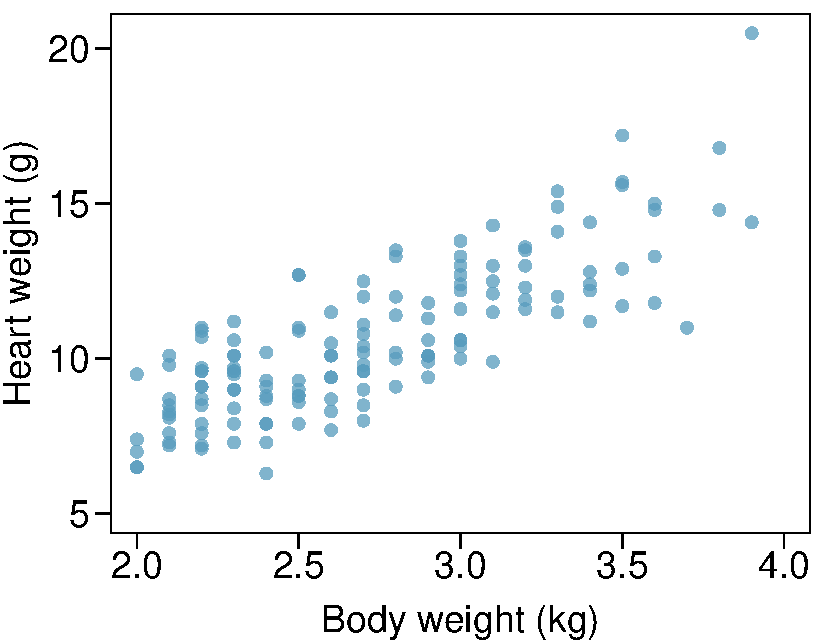
\includegraphics[width=\textwidth]{ch_simple_linear_regression_oi_biostat/figures/eoce/cat_body_heart_reg/cat_body_heart.pdf}
\end{minipage}
}{}

% oibio 12
% oi4 27

\eoce{\qt{Outliers, Part I\label{outliers_1}} Identify the outliers in the 
scatterplots shown below, and determine what type of outliers they are. 
Explain your reasoning.
\begin{center}
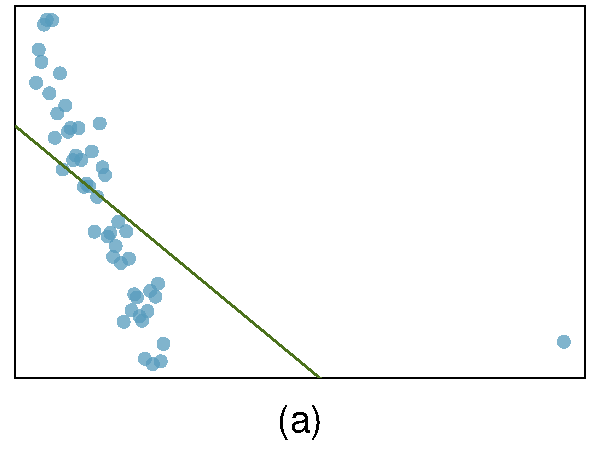
\includegraphics[width=0.32\textwidth]{ch_simple_linear_regression_oi_biostat/figures/eoce/outliers_1/outliers_1_influential.pdf}
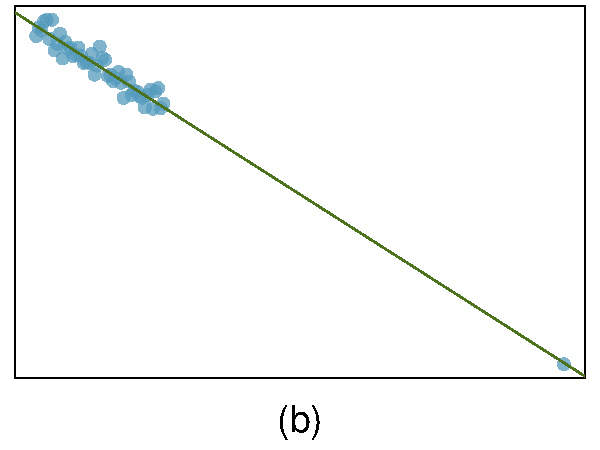
\includegraphics[width=0.32\textwidth]{ch_simple_linear_regression_oi_biostat/figures/eoce/outliers_1/outliers_2_leverage.pdf}
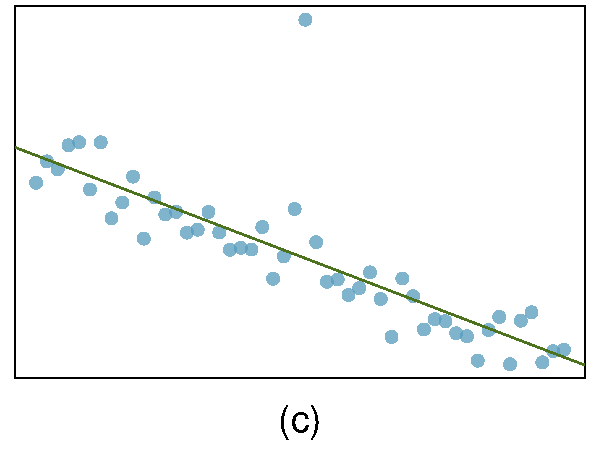
\includegraphics[width=0.32\textwidth]{ch_simple_linear_regression_oi_biostat/figures/eoce/outliers_1/outliers_3_outlier.pdf}
\end{center}
}{}

% oibio 13
% oi4 28

\eoce{\qt{Outliers, Part II\label{outliers_2}} Identify the outliers in the scatterplots 
shown below and determine what type of outliers they are. Explain 
your reasoning.
\begin{center}
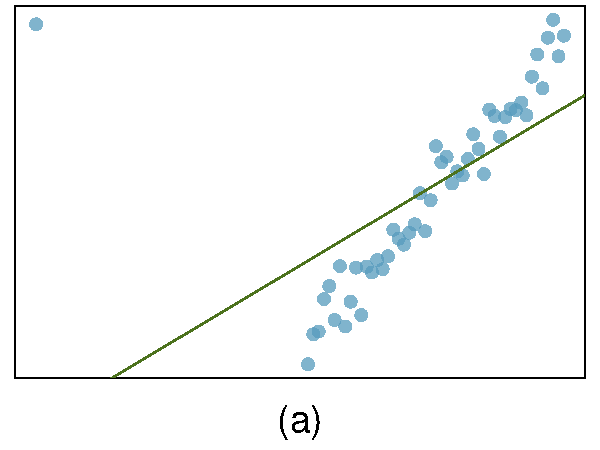
\includegraphics[width=0.32\textwidth]{ch_simple_linear_regression_oi_biostat/figures/eoce/outliers_2/outliers_1_influential.pdf}
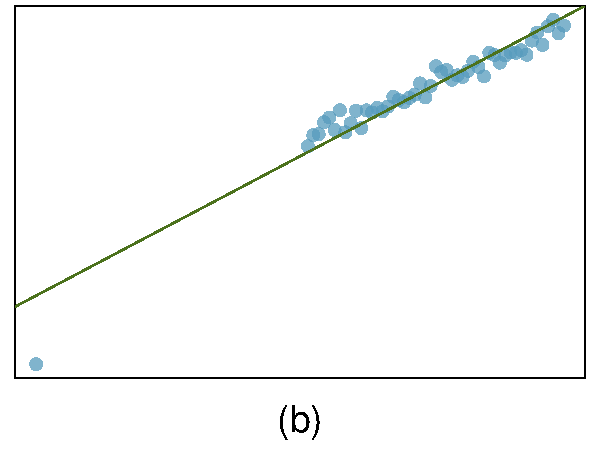
\includegraphics[width=0.32\textwidth]{ch_simple_linear_regression_oi_biostat/figures/eoce/outliers_2/outliers_2_influential.pdf}
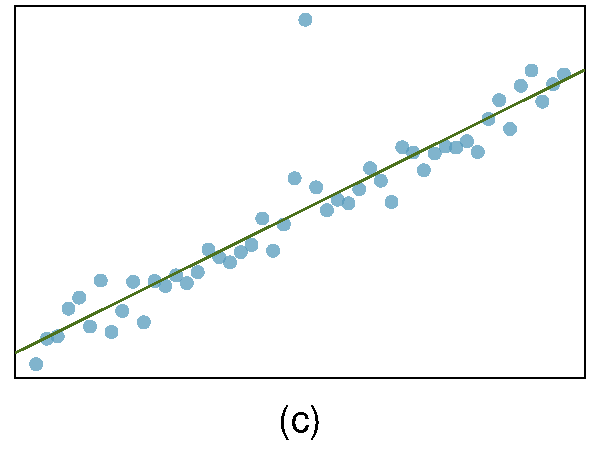
\includegraphics[width=0.32\textwidth]{ch_simple_linear_regression_oi_biostat/figures/eoce/outliers_2/outliers_3_outlier.pdf}
\end{center}
}{}

% oibio 14
% oi4 31

\eoce{\qt{Body measurements, Part IV\label{body_measurements_weight_height_inf}} 
The scatterplot and least squares summary below show the relationship 
between weight measured in kilograms and height measured in centimeters 
of 507 physically active individuals.

\noindent\begin{minipage}[c]{0.4\textwidth}
\begin{center}
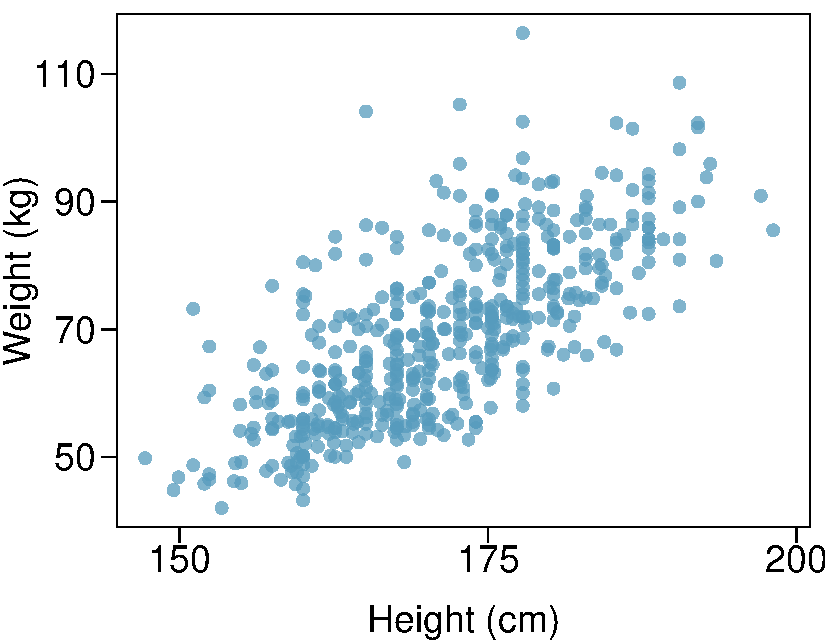
\includegraphics[width=\textwidth]{ch_simple_linear_regression_oi_biostat/figures/eoce/body_measurements_weight_height_inf/body_measurements_weight_height.pdf}
\end{center}
\end{minipage}
\begin{minipage}[c]{0.6\textwidth}
{\scriptsize
\begin{center}
\begin{tabular}{rrrrr}
    \hline
            & Estimate  & Std. Error    & t value   & Pr($>$$|$t$|$) \\ 
    \hline
(Intercept) & -105.0113 & 7.5394        & -13.93    & 0.0000 \\ 
height      & 1.0176    & 0.0440        & 23.13     & 0.0000 \\
    \hline
\end{tabular}
\end{center}
}
\end{minipage}
\begin{parts}
\item Describe the relationship between height and weight.
\item Write the equation of the regression line. Interpret the slope 
and intercept in context.
\item Do the data provide strong evidence that an increase in height 
is associated with an increase in weight? State the null and alternative 
hypotheses, report the p-value, and state your conclusion.
\item The correlation coefficient for height and weight is 0.72. 
Calculate $R^2$ and interpret it in context.
\end{parts}
}{}

% oibio 15
% oi4 32

\eoce{\qt{Beer and blood alcohol content\label{beer_blood_alcohol_inf}} 
Many people believe that gender, 
weight, drinking habits, and many other factors are much more important 
in predicting blood alcohol content (BAC) than simply considering the 
number of drinks a person consumed. Here we examine data from sixteen 
student volunteers at Ohio State University who each drank a randomly 
assigned number of cans of beer. These students were evenly divided 
between men and women, and they differed in weight and drinking habits. 
Thirty minutes later, a police officer measured their blood alcohol 
content (BAC) in grams of alcohol per deciliter of blood.
\footfullcite{Malkevitc+Lesser:2008} The scatterplot and regression 
table summarize the findings.

\noindent\begin{minipage}[c]{0.4\textwidth}
\begin{center}
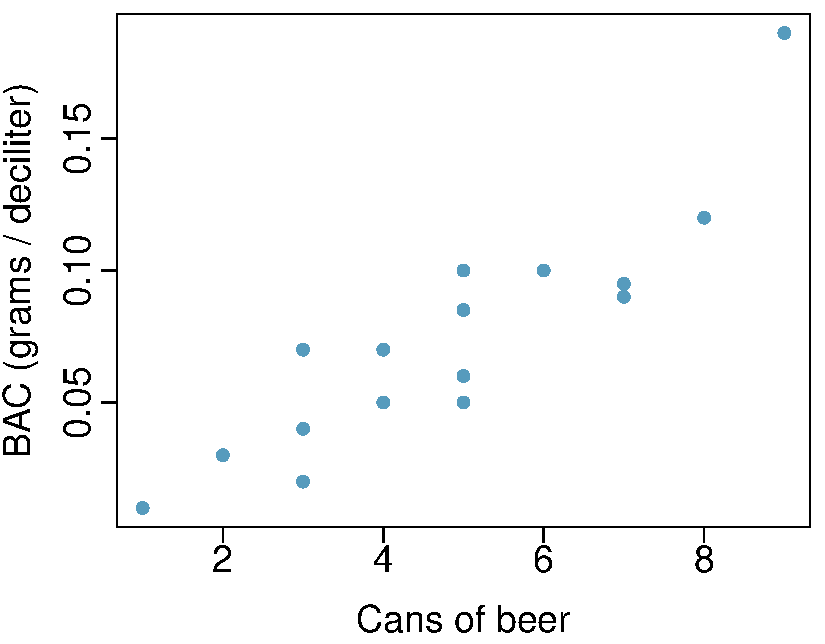
\includegraphics[width=\textwidth]{ch_simple_linear_regression_oi_biostat/figures/eoce/beer_blood_alcohol_inf/beer_blood_alcohol.pdf}
\end{center}
\end{minipage}
\begin{minipage}[c]{0.6\textwidth}
{\scriptsize
\begin{center}
\begin{tabular}{rrrrr}
    \hline
            & Estimate  & Std. Error    & t value   & Pr($>$$|$t$|$) \\ 
    \hline
(Intercept) & -0.0127   & 0.0126        & -1.00     & 0.3320 \\ 
beers       & 0.0180    & 0.0024        & 7.48      & 0.0000 \\ 
    \hline
\end{tabular}
\end{center}
}
\end{minipage}
\begin{parts}
\item Describe the relationship between the number of cans of beer 
and BAC.
\item Write the equation of the regression line. Interpret the slope 
and intercept in context.
\item Do the data provide strong evidence that drinking more cans of 
beer is associated with an increase in blood alcohol? State the null 
and alternative hypotheses, report the p-value, and state your 
conclusion.
\item The correlation coefficient for number of cans of beer and BAC 
is 0.89. Calculate $R^2$ and interpret it in context.
\item Suppose we visit a bar, ask people how many drinks they have had, 
and also take their BAC. Do you think the relationship between number 
of drinks and BAC would be as strong as the relationship found in the 
Ohio State study?
\end{parts}
}{}

%\D{\newpage}

% oibio 16
% oi4 33

\eoce{\qt{Husbands and wives, Part II\label{husbands_wives_height_inf}} The 
scatterplot below summarizes husbands' and wives' heights in a random 
sample of 170 married couples in Britain, where both partners' ages are 
below 65 years. Summary output of the least squares fit for predicting 
wife's height from husband's height is also provided in the table.

\noindent\begin{minipage}[c]{0.4\textwidth}
\begin{center}
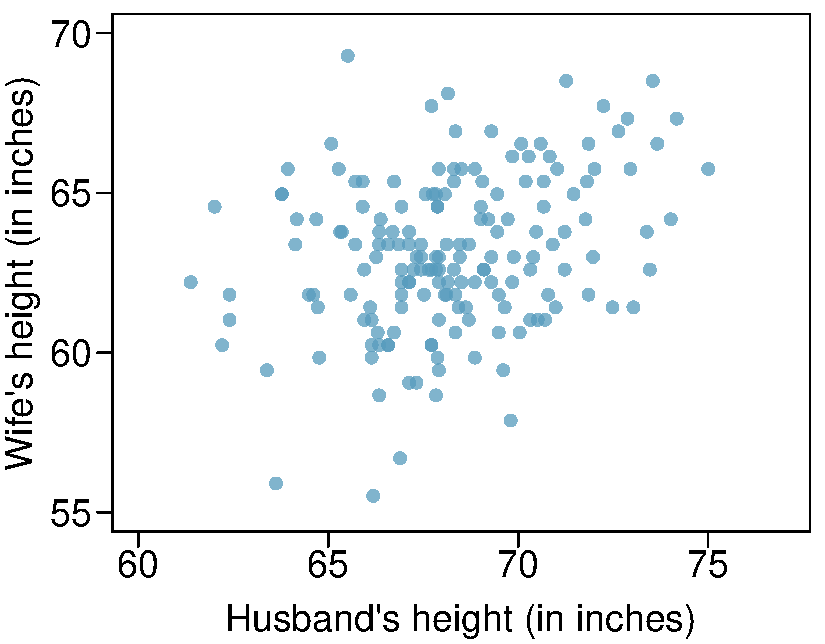
\includegraphics[width=\textwidth]{ch_simple_linear_regression_oi_biostat/figures/eoce/husbands_wives_height_inf_2s/husbands_wives_height_inf_2s}
\end{center}
\end{minipage}
\begin{minipage}[c]{0.6\textwidth}
{\scriptsize
\begin{center}
\begin{tabular}{rrrrr}
    \hline
                    & Estimate  & Std. Error    & t value   & Pr($>$$|$t$|$) \\ 
    \hline
(Intercept)         & 43.5755   & 4.6842        & 9.30      & 0.0000 \\ 
height\_\hspace{0.3mm}husband   & 0.2863    & 0.0686        & 4.17      & 0.0000 \\ 
    \hline
\end{tabular}
\end{center}
}
\end{minipage}
\begin{parts}
\item Is there strong evidence that taller men marry taller women? 
State the hypotheses and include any information used to conduct the test.
\item Write the equation of the regression line for predicting wife's 
height from husband's height.
\item Interpret the slope and intercept in the context of the application.
\item Given that $R^2 = 0.09$, what is the correlation of heights 
in this data set?
\item You meet a married man from Britain who is 5'9" (69 inches). 
What would you predict his wife's height to be? How reliable is this 
prediction?
\item You meet another married man from Britain who is 6'7" (79 inches). 
Would it be wise to use the same linear model to predict his wife's 
height? Why or why not?
\end{parts}
}{}

% oibio 17
% oi4 39

\eoce{\qt{Husbands and wives, Part III\label{husbands_wives_age_inf}}
Exercise~\ref{husbands_wives_height_inf} presents a scatterplot displaying the 
relationship between husbands' and wives' ages in a random sample of 
170 married couples in Britain, where both partners' ages are below 65 
years. Given below is summary output of the least squares fit for 
predicting wife's age from husband's age.

\noindent\begin{minipage}[c]{0.4\textwidth}
\begin{center}
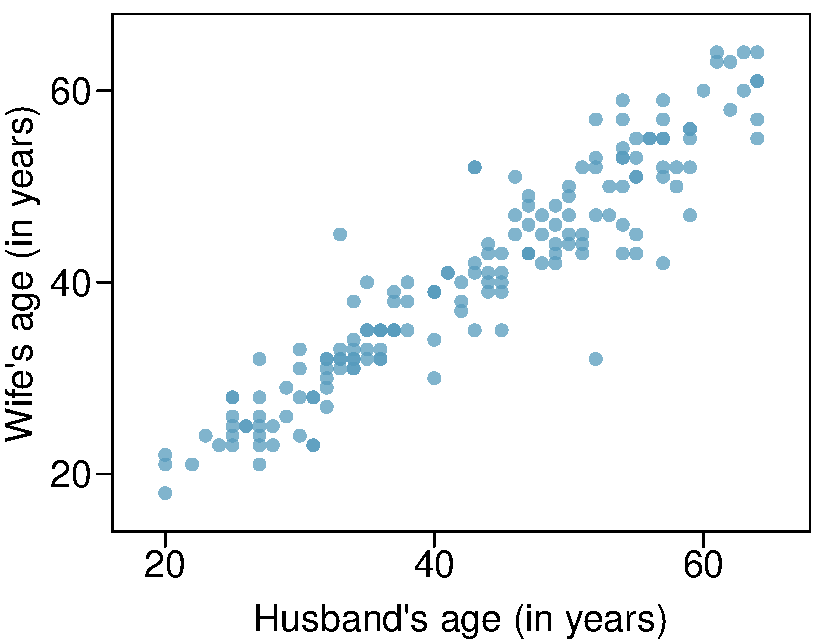
\includegraphics[width=\textwidth]{ch_simple_linear_regression_oi_biostat/figures/eoce/husbands_wives_age_inf/husbands_wives_age.pdf}
\end{center}
\end{minipage}
\begin{minipage}[c]{0.6\textwidth}
{\scriptsize
\begin{center}
\begin{tabular}{rrrrr}
  \hline
                & Estimate  & Std. Error    & t value   & Pr($>$$|$t$|$) \\ 
  \hline
(Intercept)     & 1.5740    & 1.1501        & 1.37      & 0.1730 \\ 
age\_\hspace{0.3mm}husband  & 0.9112    & 0.0259        & 35.25     & 0.0000 \\ 
   \hline
\multicolumn{5}{r}{$df = 168$} \\
\end{tabular}
\end{center}
}
\end{minipage}
\begin{parts}
\item We might wonder, is the age difference between husbands and 
wives consistent across ages? If this were the case, then the slope 
parameter would be $\beta_1 = 1$. Use the information above to evaluate 
if there is strong evidence that the difference in husband and wife ages 
differs for different ages.
\item Write the equation of the regression line for predicting wife's 
age from husband's age.
\item Interpret the slope and intercept in context.
\item Given that $R^2 = 0.88$, what is the correlation of ages  in 
this data set?
\item You meet a married man from Britain who is 55 years old. What 
would you predict his wife's age to be? How reliable is this prediction?
\item You meet another married man from Britain who is 85 years old. 
Would it be wise to use the same linear model to predict his wife's 
age? Explain.
\end{parts}
}{}

% oibio 18
% 41

\eoce{\qt{Nutrition at Starbucks, Part II\label{starbucks_cals_protein}} 
Exercise~\ref{starbucks_cals_carbos} introduced a data set on nutrition 
information on Starbucks food menu items. Based on the scatterplot 
and the residual plot provided, describe the relationship between the 
protein content and calories of these menu items, and determine if a 
simple linear model is appropriate to predict amount of protein from 
the number of calories.
\begin{center}
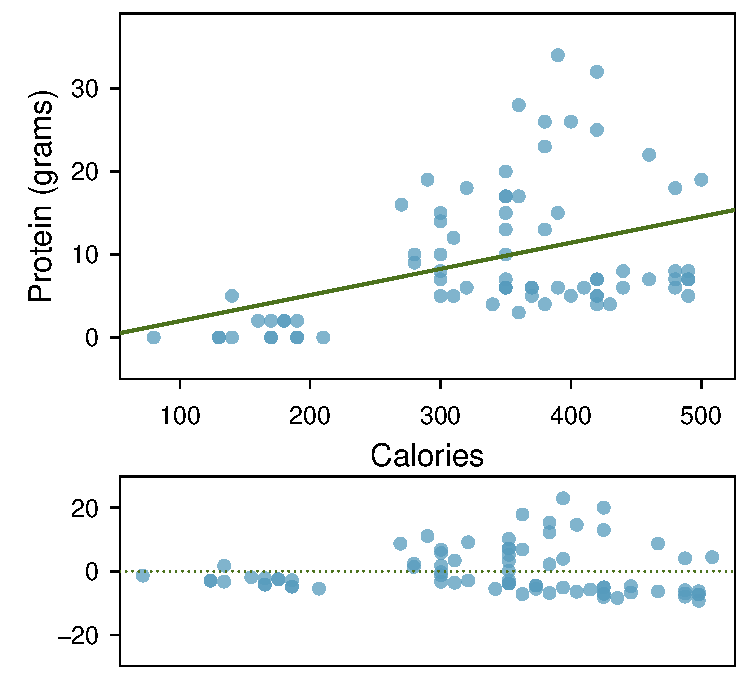
\includegraphics[width=0.35\textwidth]{ch_simple_linear_regression_oi_biostat/figures/eoce/starbucks_cals_protein/starbucks_cals_protein}
\end{center}
}{}

% oibio 19
% oi4 42

\eoce{\qt{Helmets and lunches\label{helmet_lunch}}
The scatterplot shows the 
relationship between socioeconomic status measured as the percentage of 
children in a neighborhood receiving reduced-fee lunches at school 
({\tt lunch}) and the percentage of bike riders in the neighborhood 
wearing helmets ({\tt helmet}). The average percentage of children 
receiving reduced-fee lunches is 30.8\% with a standard deviation 
of 26.7\% and the average percentage of bike riders wearing helmets 
is 38.8\% with a standard deviation of 16.9\%.

\noindent\begin{minipage}[c]{0.5\textwidth}
{\raggedright\begin{parts}
\item If the $R^2$ for the least-squares regression line for these 
data is $72\%$, what is the correlation between {\tt lunch} 
and {\tt helmet}?
\item Calculate the slope and intercept for the least-squares regression 
line for these data.
\item Interpret the intercept of the least-squares regression line in 
the context of the application.
\item Interpret the slope of the least-squares regression line in the 
context of the application.
\item What would the value of the residual be for a neighborhood where 
40\% of the children receive reduced-fee lunches and 40\% of the bike 
riders wear helmets? Interpret the meaning of this residual in the context 
of the application.
\end{parts}}
\end{minipage}
\begin{minipage}[c]{0.05\textwidth}
$\:$ \\
\end{minipage}
\begin{minipage}[c]{0.42\textwidth}
\begin{center}
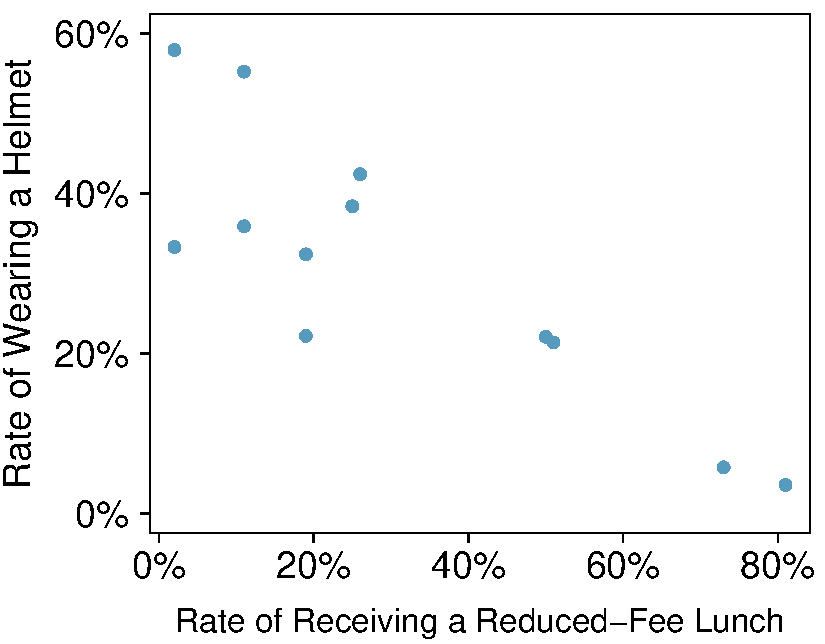
\includegraphics[width=\textwidth]{ch_simple_linear_regression_oi_biostat/figures/eoce/helmet_lunch/helmet_lunch.pdf} \\
\end{center}
\end{minipage}
}{}



